\documentclass[12pt]{article}
\usepackage{lmodern}
\usepackage{hyperref}
\usepackage{setspace}
\usepackage{float}
\hypersetup{
	colorlinks,
	citecolor=black,
	filecolor=black,
	linkcolor=black,
	urlcolor=black	
}
\usepackage{amsmath}
\usepackage{listings}
\usepackage{graphicx}
\usepackage{subcaption} 
\usepackage{caption}
\usepackage{geometry}
\usepackage{enumerate}
\usepackage{array, booktabs}  
\geometry{
	a4paper ,
	total={170mm,257mm},
	left=23mm,
	top=25mm,
	bottom = 25mm,
	right = 23mm
}	
\usepackage{fancyhdr}
\usepackage{gensymb}
\pagestyle{fancy}
\DeclareGraphicsExtensions{.jpg,.png,.pdf}

\usepackage{anyfontsize}

\lhead{}
\chead {ANLP Assignment 1}
\rhead{}
\cfoot{\thepage}

\usepackage[utf8]{inputenc}
\usepackage{color}

\definecolor{codegreen}{rgb}{0,0.6,0}
\definecolor{codegray}{rgb}{0.5,0.5,0.5}
\definecolor{codepurple}{rgb}{0.58,0,0.82}
\definecolor{backcolour}{rgb}{1,1,1}

\lstdefinestyle{mystyle}{
	backgroundcolor=\color{backcolour},   
	commentstyle=\color{codegreen},
	keywordstyle=\color{blue},
	numberstyle=\tiny\color{codegray},
	stringstyle=\color{codepurple},
	basicstyle=\footnotesize,
	breakatwhitespace=false,         
	breaklines=true,                 
	captionpos=b,                    
	keepspaces=true,                 
	numbers=left,                    
	numbersep=5pt,                  
	showspaces=false,                
	showstringspaces=false,
	showtabs=false,                  
	tabsize=2
}
\lstset{style=mystyle}


\usepackage{algorithm}
\usepackage[noend]{algpseudocode}

\makeatletter
\def\BState{\State\hskip-\ALG@thistlm}
\makeatother

\usepackage[nottoc,numbib]{tocbibind}

\setlength{\arrayrulewidth}{1mm}
\setlength{\tabcolsep}{18pt}
\renewcommand{\arraystretch}{1.5}
% To Dos:
% Add comments to code - place comments on inputs/outputs of functions too apparently


\begin{document}	
	
\begin{titlepage}
	\newcommand{\HRule}{\rule{\linewidth}{0.5mm}} % Defines a new command for the horizontal lines, change thickness here
	\center % Center everything on the page
	\includegraphics[width = 0.3 \linewidth]{"./graphics/avatar-roundel-blackonwhite"}\\[0.5cm]
	\textsc{\\[1cm]\LARGE ACCELERATED NATURAL LANGUAGE \\
             \hfill\break PROCESSING}\\[2cm]

	\HRule \\[0.4cm]
	{ \huge \bfseries Assignment 1}\\[0.1cm]
	\HRule \\[1.5cm]
	\Large
	\vfill
	 S1818699, S1884908\\[0.5cm]
	{\large July 2018}
\end{titlepage}
\setlength\parindent{0pt}		
\newpage
\doublespacing
\tableofcontents
\singlespacing
\newpage
	
\section{Introduction}

\section{Random Sequence Generation - Question 4}
\subsection{Raw Application of Language Model}
After having generated and built a language model, the model itself can be used as is to generate new sequences.
\subsection{Random generation}
\begin{algorithm}
	\caption{Random Generation}\label{RanGen}
	\begin{algorithmic}[1]
		\Procedure{generate\_from\_lm}{Num\_Chars, Model, Valid\_Char\_List}
		\State $sequence = empty$
		\State $bigram\_in \gets  \text{`\#'} + random(Valid\_Char\_List)$
		\State $chars\_left \gets Num\_Chars -1$
		\BState \emph{loop}:
		\If {$chars\_left > 0$}
		\State $pos\_tris \gets [bigram\_in + Valid\_Char\_List]$.
		\State $distribution \gets model[pos\_tris]$.
		\State $bins \gets cumulative sum(distribution)$
		\State $seq\_pos \gets random\_bin\_select(bins)$
		\State $new\_seq \gets pos\_tris[seq\_pos]$
		\State $bigram\_in \gets new\_seq[0:1]$
		\State $sequence \gets sequence + new\_seq[2]$
		\State $chars\_left \gets chars\_left - 1$
		\State \textbf{goto} \emph{loop}.
		\EndIf
		\State \textbf{return} $sequence$
		\EndProcedure
	\end{algorithmic}
\end{algorithm}
\begin{figure}[H]
	\centering
	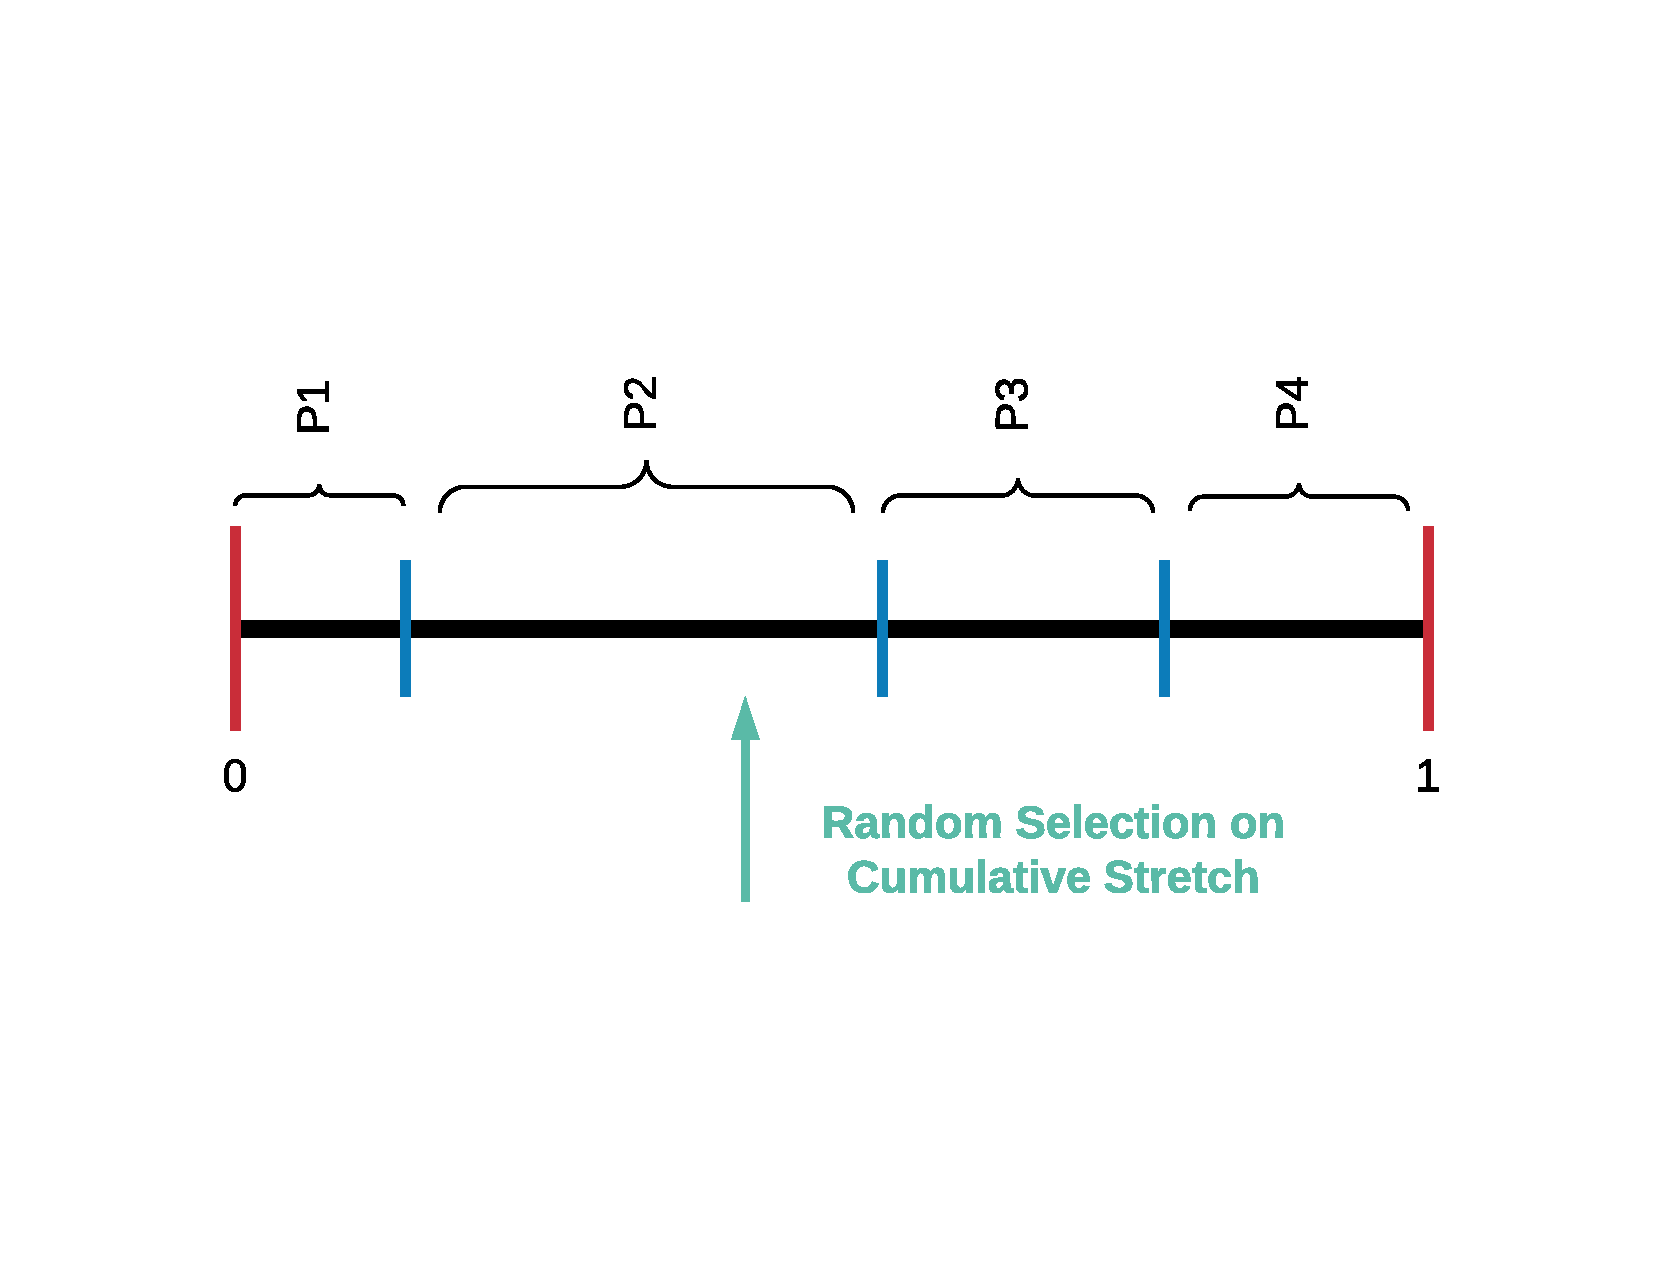
\includegraphics[width=0.7\linewidth]{graphics/Random_Gen}
	\caption{Random selection from a probability distribution}
	\label{fig:randomgen}
\end{figure}

\subsection{Results}

\section{Perplexity Computation - Question 5}
This part of the assignment dealt with utilising the generated language models to assess the content of a given text.
\subsection{Perplexity Computation}
A perplexity measure attempt to measure how well a given model predicts a selected text sample.  A low perplexity indicates the model is well suited to predicting the selected text, whilst a high perplexity indicates the model is unsuited for the text selected.  The general equation for perplexity computation is as follows:
\begin{equation}
	PP_{M} = P_{M}\left( w_{1}.... w_{n}\right)^{-\frac{1}{n}}
\end{equation}
Taking logs:
\begin{equation}
log\left(PP_{M}\right) = log\left(P_{M}\left( w_{1}.... w_{n}\right)^{-\frac{1}{n}}\right)
\end{equation}
\begin{equation}
log\left(PP_{M}\right) = -\frac{1}{n}\times log\left(P_{M}\left( w_{1}.... w_{n}\right)\right)
\end{equation}
\begin{equation}
log\left(PP_{M}\right) = -\frac{1}{n} \sum_{i=1} ^{n}\left( log(P_{M}(w_{1})) + ... + log(P_{M}(w_{n})) \right)
\end{equation}
\subsection{Test Results}



\subsection{Document Language Determination}
Following the categorisation of the 
%read in a doc and  test perplex.
%perplexity of test doc under all language models
%how to use numbers to guess language
% if used on a random file, enough to guess if english?
%


\section{Conclusions}

\end{document}
